%Version 3.1 December 2024
% See section 11 of the User Manual for version history
%
%%%%%%%%%%%%%%%%%%%%%%%%%%%%%%%%%%%%%%%%%%%%%%%%%%%%%%%%%%%%%%%%%%%%%%
%%                                                                 %%
%% Please do not use \input{...} to include other tex files.       %%
%% Submit your LaTeX manuscript as one .tex document.              %%
%%                                                                 %%
%% All additional figures and files should be attached             %%
%% separately and not embedded in the \TeX\ document itself.       %%
%%                                                                 %%
%%%%%%%%%%%%%%%%%%%%%%%%%%%%%%%%%%%%%%%%%%%%%%%%%%%%%%%%%%%%%%%%%%%%%

%%\documentclass[referee,sn-basic]{sn-jnl}% referee option is meant for double line spacing

%%=======================================================%%
%% to print line numbers in the margin use lineno option %%
%%=======================================================%%

%%\documentclass[lineno,pdflatex,sn-basic]{sn-jnl}% Basic Springer Nature Reference Style/Chemistry Reference Style

%%=========================================================================================%%
%% the documentclass is set to pdflatex as default. You can delete it if not appropriate.  %%
%%=========================================================================================%%

%%\documentclass[sn-basic]{sn-jnl}% Basic Springer Nature Reference Style/Chemistry Reference Style

%%Note: the following reference styles support Namedate and Numbered referencing. By default the style follows the most common style. To switch between the options you can add or remove “Numbered” in the optional parenthesis. 
%%The option is available for: sn-basic.bst, sn-chicago.bst%  
 
%%\documentclass[pdflatex,sn-nature]{sn-jnl}% Style for submissions to Nature Portfolio journals
%%\documentclass[pdflatex,sn-basic]{sn-jnl}% Basic Springer Nature Reference Style/Chemistry Reference Style
\documentclass[pdflatex,sn-mathphys-num]{sn-jnl}% Math and Physical Sciences Numbered Reference Style
%%\documentclass[pdflatex,sn-mathphys-ay]{sn-jnl}% Math and Physical Sciences Author Year Reference Style
%%\documentclass[pdflatex,sn-aps]{sn-jnl}% American Physical Society (APS) Reference Style
%%\documentclass[pdflatex,sn-vancouver-num]{sn-jnl}% Vancouver Numbered Reference Style
%%\documentclass[pdflatex,sn-vancouver-ay]{sn-jnl}% Vancouver Author Year Reference Style
%%\documentclass[pdflatex,sn-apa]{sn-jnl}% APA Reference Style
%%\documentclass[pdflatex,sn-chicago]{sn-jnl}% Chicago-based Humanities Reference Style

%%%% Standard Packages
%%<additional latex packages if required can be included here>

\usepackage{graphicx}%
\usepackage{multirow}%
\usepackage{amsmath,amssymb,amsfonts}%
\usepackage{amsthm}%
\usepackage{mathrsfs}%
\usepackage[title]{appendix}%
\usepackage{xcolor}%
\usepackage{textcomp}%
\usepackage{manyfoot}%
\usepackage{booktabs}%
\usepackage{algorithm}%
\usepackage{algorithmicx}%
\usepackage{algpseudocode}%
\usepackage{listings}%
\usepackage{indentfirst}
\usepackage{placeins}
%%%%

%%%%%=============================================================================%%%%
%%%%  Remarks: This template is provided to aid authors with the preparation
%%%%  of original research articles intended for submission to journals published 
%%%%  by Springer Nature. The guidance has been prepared in partnership with 
%%%%  production teams to conform to Springer Nature technical requirements. 
%%%%  Editorial and presentation requirements differ among journal portfolios and 
%%%%  research disciplines. You may find sections in this template are irrelevant 
%%%%  to your work and are empowered to omit any such section if allowed by the 
%%%%  journal you intend to submit to. The submission guidelines and policies 
%%%%  of the journal take precedence. A detailed User Manual is available in the 
%%%%  template package for technical guidance.
%%%%%=============================================================================%%%%

%% as per the requirement new theorem styles can be included as shown below
\theoremstyle{thmstyleone}%
\newtheorem{theorem}{Theorem}%  meant for continuous numbers
%%\newtheorem{theorem}{Theorem}[section]% meant for sectionwise numbers
%% optional argument [theorem] produces theorem numbering sequence instead of independent numbers for Proposition
\newtheorem{proposition}[theorem]{Proposition}% 
%%\newtheorem{proposition}{Proposition}% to get separate numbers for theorem and proposition etc.

\theoremstyle{thmstyletwo}%
\newtheorem{example}{Example}%
\newtheorem{remark}{Remark}%

\theoremstyle{thmstylethree}%
\newtheorem{definition}{Definition}%

\raggedbottom
%%\unnumbered% uncomment this for unnumbered level heads

\begin{document}

\title[Article Title]{Mudança climática: Análise exploratória das condições de temperatura e precipitação da estação A705 do INMET em Bauru (2002–2025)}

%%=============================================================%%
%% GivenName	-> \fnm{Joergen W.}
%% Particle	-> \spfx{van der} -> surname prefix
%% FamilyName	-> \sur{Ploeg}
%% Suffix	-> \sfx{IV}
%% \author*[1,2]{\fnm{Joergen W.} \spfx{van der} \sur{Ploeg} 
%%  \sfx{IV}}\email{iauthor@gmail.com}
%%=============================================================%%

\author*[1]{\fnm{Gabriel} \sur{Naka}}\email{gabriel.naka@unesp.br}
\equalcont{}

\author*[1]{\fnm{Thiago} \sur{Toreto}}\email{thiago.toreto@unesp.br}
\equalcont{\textbf{Esses autores countribuiram igualmente para esse trabalho.}}

%\author[1,2]{\fnm{Third} \sur{Author}}\email{iiiauthor@gmail.com}
%\equalcont{These authors contributed equally to this work.}

\affil*[1]{\orgdiv{Bacharelado em Ciência da Computação}, \orgname{UNESP}, \orgaddress{\street{Av. Eng. Luís Edmundo Carrijo Coube, 14-01 - Vargem Limpa}, \city{Bauru}, \postcode{17033-360}, \state{São Paulo}, \country{Brasil}}}

%\affil[2]{\orgdiv{Department}, \orgname{Organization}, \orgaddress{\street{Street}, \city{City}, \postcode{10587}, \state{State}, \country{Country}}}

%\affil[3]{\orgdiv{Department}, \orgname{Organization}, \orgaddress{\street{Street}, \city{City}, \postcode{610101}, \state{State}, \country{Country}}}

%%==================================%%
%% Sample for unstructured abstract %%
%%==================================%%

%\abstract{The abstract serves both as a general introduction to the topic and as a brief, non-technical summary of the main results and their implications. Authors are advised to check the author instructions for the journal they are submitting to for word limits and if structural elements like subheadings, citations, or equations are permitted.}

\abstract{Esse trabalho busca realizar uma \textit{análise exploratória de dados}(EDA) para analisar série histórica de condições meteorológicas de temperatura e precipitação providas por medições horárias da estação automática A705, localizada em Bauru(SP), construída e mantida pelo Instituto Nacional de Meteorologia(INMET), considerando as observações dos anos de 2002 a 2025. A análise tem como objetivo confirmar ou rejeitar estatisticamente a possibilidade de mudanças significativas das condições climáticas da região, e considerar como o resultado impactaria decisões de planejamento de infraestrutura local. O trabalho conclui que há razão para preparar a infraestrutura para aumentos de temperatura no futuro, mas que essas previsões não são absolutas e mais estudos são necessários }

%%================================%%
%% Sample for structured abstract %%
%%================================%%

% \abstract{\textbf{Purpose:} The abstract serves both as a general introduction to the topic and as a brief, non-technical summary of the main results and their implications. The abstract must not include subheadings (unless expressly permitted in the journal's Instructions to Authors), equations or citations. As a guide the abstract should not exceed 200 words. Most journals do not set a hard limit however authors are advised to check the author instructions for the journal they are submitting to.
% 
% \textbf{Methods:} The abstract serves both as a general introduction to the topic and as a brief, non-technical summary of the main results and their implications. The abstract must not include subheadings (unless expressly permitted in the journal's Instructions to Authors), equations or citations. As a guide the abstract should not exceed 200 words. Most journals do not set a hard limit however authors are advised to check the author instructions for the journal they are submitting to.
% 
% \textbf{Results:} The abstract serves both as a general introduction to the topic and as a brief, non-technical summary of the main results and their implications. The abstract must not include subheadings (unless expressly permitted in the journal's Instructions to Authors), equations or citations. As a guide the abstract should not exceed 200 words. Most journals do not set a hard limit however authors are advised to check the author instructions for the journal they are submitting to.
% 
% \textbf{Conclusion:} The abstract serves both as a general introduction to the topic and as a brief, non-technical summary of the main results and their implications. The abstract must not include subheadings (unless expressly permitted in the journal's Instructions to Authors), equations or citations. As a guide the abstract should not exceed 200 words. Most journals do not set a hard limit however authors are advised to check the author instructions for the journal they are submitting to.}


\keywords{Análise exploratória de dados, mudança climática, INMET, Bauru, temperatura, precipitação, planejamento urbano }

%%\pacs[JEL Classification]{D8, H51}

%%\pacs[MSC Classification]{35A01, 65L10, 65L12, 65L20, 65L70}


\maketitle

\newpage
\renewcommand*\contentsname{Sumário}
\tableofcontents
\newpage

\section{Introdução}\label{sec1}

O planejamento urbano e a construção de infraestrutura são fortemente afetados pelas condições climáticas presentes e a longo prazo da região.  Temperatura, chuva, períodos secos e eventos intensos interferem, entre outros aspectos, no conforto térmico, na arborização, na drenagem, no planejamento de recursos hídricos, assim como escolha de materias e planejamento de reparos e obras. Nesse contexto, governos regionais são fortemente incentivados a conhecer, não só as características climaticas presentes, mas também as tendências de modificação dessas condições para que a infraestrutura urbana seja efetiva a longo prazo.

Considerando esses fatores, a prefeitura municipal de Bauru, São Paulo, demonstrou interesse em realizar um estudo EDA a respeito das condições meteorológicas de temperatura e precipitação da região para melhor poder realizar decisões de planejamento urbano a médio e longo prazo.

Portanto, esse trabalho busca realizar uma análise para estudar essa possibilidade da existência de tendências significativas de mudanças climáticas, e comprová-las ou disprová-las estatisticamente. O escopo do estudo se delimitou às leituras horárias disponibilizadas pelo portal INMET(Instituto Nacional de Meteorologia)\cite{bib1} relativos aos anos completos de 2002 a 2025 coletados pela estação automática A705, localizada no lado sul da cidade de Bauru, em proximidade ao Departamento de Educação Física da Universidade Estadual Paulista "Júlio de Mesquita Filho"(UNESP), como visto na imagem \ref{fig:mapa}.

A delimitação temporal aos anos de 2002 a 2025 ocorreu, apesar da base de dados oferecer leituras dos anos de 2000 a 2026, pois foram nesses anos que a estação sob estudo realizou leituras durante todos os períodos do ano, com 2000 não apresentando dados, e com 2001 e 2026 não apresentando  dados de todos os meses. O delimitamento espacial da estação A705, por sua vez, foi causado pela inadequação das outras estações, causadas por fatores como menor variabilidade de dados coletados, menor tempo de funcionamento, ou diferenças geográficas as tornarem menos consistentes e relevantes à ánalise em questão. 
Algumas das estações consideradas estão mostradas na imagem \ref{fig:estacoes}, contendo as localidades das estações, código de identificação, distância até o ponto primário A705, assim como o primeiro ano onde a estação esteve ativa durante todos os períodos do ano. A figura representa todas estações\cite{bib2} com distância de Bauru inferior a 100km, e demonstra, além dessa quantidade ser pequena, as estações apresentam significativamente menos anos completos, fato que prejudicaria severamente o estudo ao reduzir o período em que podem ser detectadas tendências, reduzindo precisão.

A execução dessa pesquisa será realizada primáriamente atráves de programas em linguagem \textit{Python}, em conjunto com \textit{Jupyter Notebook} para organizar e documentar os códigos, o qual serão disponibilizados e versionados atráves de repositórios \textit{GitHub}.

\begin{figure}[htbp]
    \centering
    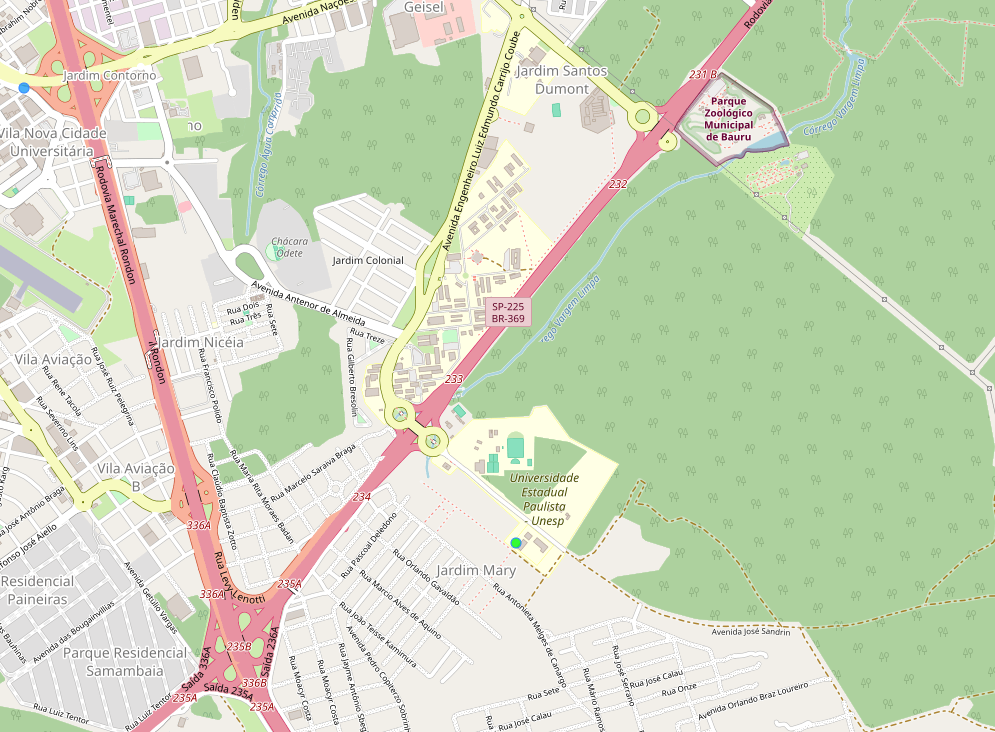
\includegraphics[width=0.9\textwidth]{figs/map.png}
    \caption{Mapa provido pelo INMET, com a estação A705 marcada com um circulo verde.}
    \label{fig:mapa}
\end{figure}

\begin{figure}[htbp]
    \centering
    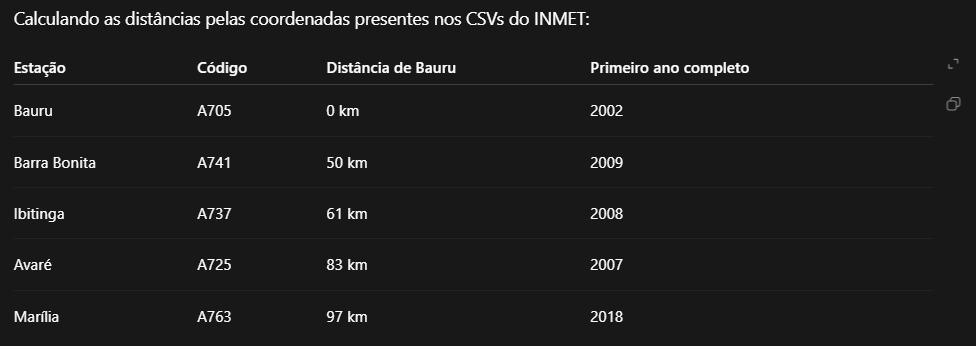
\includegraphics[width=\textwidth]{figs/estacoes.jpeg}
    \caption{Lista de estações com distância menor de 100km para A705, com primeiro ano completo.}
    \label{fig:estacoes}
\end{figure}

\clearpage


\section{Desenvolvimento}\label{sec2}

\subsection{Fonte de Dados}

Na fonte de dados, portal INMET, são disponibilizados arquivos compactados por ano, de 2000 a 2026, contendo nesses arquivos .csv(comma-separated values), como visto na imagem \ref{fig:exemploBruto}, contendo, individualmente, dados de identificador, localização administrativa e geográfica da estação automática, assim como dados de precipitação, pressão, radiação, temperatura, umidade e ventos, coletados idealmente a cada hora durante todo o ano.

Esses dados, porém, não foram coletados e catalogados perfeitamente, notando-se que um número extremamente pequeno de estações possuem dados em 2000, apenas 5, com nenhuma dessas possuindo dados anteriores a maio do mesmo ano, em comparação com 2026, o qual possui leituras automáticas de 639 estações. Também foi percebido que uma parcela das medições continha valores númericos absurdos ou impossíveis, de -9999, notando ausência dessa medição na especifica data, horario e local.

Outros problemas menores detectados foram leves inconsistências na nomenclatura de colunas, ambas internas e entre tabelas, diferenças nas organizações de diretórios dos dados baixados, e também arquivos com tamanhos maiores que suportados pelo repositório utilizado, GitHub.

Os problemas de consistência e completude dos dados serão tratados nos próximos tópicos, porém a equipe optou por não diretamente solucionar a dificuldade de publicar os dados de entrada através do repositório escolhido, dando outros pesquisadores a tarefa de realizar o download desses caso queiram reproduzir a análise, com o objetivo de causar com que estudos futuros sejam feitos com dados mais atualizados, destacando-se que as leituras do ano de 2026 não estavam completas pois o estudo foi realizado antes desse ano ter se completado, assim como possibilitar maior grau de confiança da veracidade dos dados.


\begin{figure}[htbp]
    \centering
    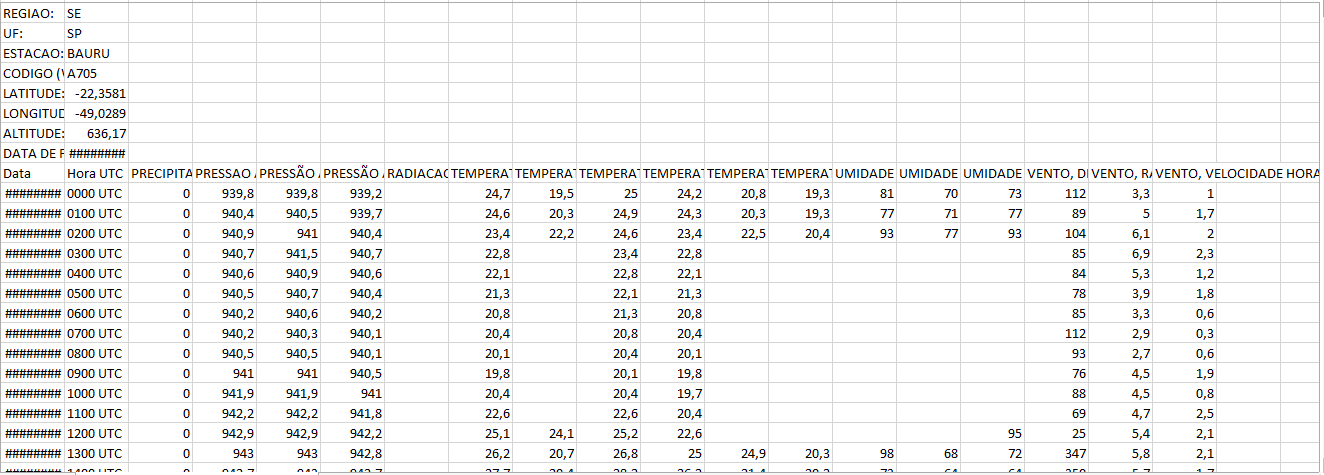
\includegraphics[width=\textwidth]{figs/exemploBruto.png}
    \caption{Exemplo de organização dos arquivos brutos de dados, ano de 2025.}
    \label{fig:exemploBruto}
\end{figure}

\FloatBarrier



\subsection{Processamento de Dados}

\subsubsection{Normalização e Consolidação}

O primeiro passo de manipulação e tratamento dos dados de observações meteorológicas envolveu padronizações diversas de nomenclatura das variáveis e suas unidades.

Nesse passo, inicialmente, são localizados todos os arquivos relevantes à estação A705 através de uma busca recursiva pela string \textit{"A705\_BAURU"}, comum a todos os arquivos desejados, solucionando inconsistências de organização e nomenclatura dos arquivos, dado que as tabelas de observações estavam inconsistentemente dentro de um ou dois diretórios de profundidade do arquivo anual baixado, e eram nomeados com as datas de primeira e última observação. Através do nome, é determinado o ano de coleta dos dados, e identificado quais estão faltantes.

Em seguida, houve a renomeação de todas as colunas relevantes dos arquivos para o mesmo formato utilizando prefixos comuns, manualmente selecionados, entre mesmas medidas de diferentes anos. Por fim dados com valores de \textit{-9999} e \textit{-9999.0} são substituidos constantes \textit{nan}

A verificação da execução correta das etapas anteriores ocorre pela contagem dos anos faltantes e da quantidade de colunas encontradas e extraidas, como mostrada na figura \ref{fig:padronizacao}.

Essa normalização é útil para garantir agrupamento de medidas similares, evitando que dados incorretamente armazenados afetem o resultado a pesquisa.


\begin{figure}[htbp]
    \centering
    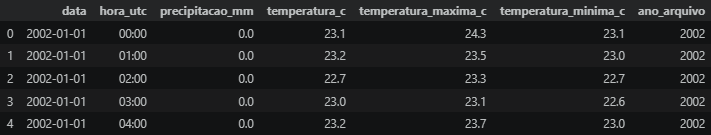
\includegraphics[width=\textwidth]{figs/padronizacao.png}
    \caption{Colunas e seus valores dos primeiros dados encontrados da estação A705 após padronização.}
    \label{fig:padronizacao}
\end{figure}

\FloatBarrier


\subsubsection{Validação das Entradas}

Para as entradas padronizadas, são então verificadas suas validades ao rejeitar possíveis valores incorretos ou falhos que não podem ser confiavelmente corrigidos ou utilizados.

As datas e horas armazenadas são convertidas para um formato padrão, como UTC, e então verificadas por valores impossíveis(negativos ou maiores que possível). As entradas válidas então recebem novas colunas para outros formatos e fusos, como em string e data local. Ao fim dessa etapa, escopo temporal é revalidado para os anos de 2002-2025, com resultados visiveis na imagem \ref{fig:UTC}.

Em seguida, valores de meteorologia altamente improváveis e impossíveis são removidos, considerando altamente improvável temperaturas menores que -10ºC e maiores que 50ºC, e impossíveis precipitações negativas e outros valores onde mínima é inferior a máxima.

\begin{figure}[htbp]
    \centering
    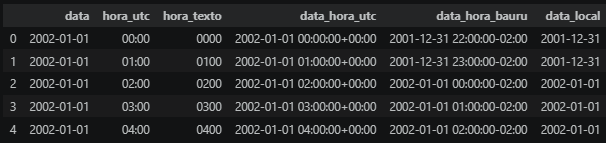
\includegraphics[width=\textwidth]{figs/UTC.png}
    \caption{Colunas e seus valores dos primeiros dados encontrados da estação A705 após conversão temporal.}
    \label{fig:UTC}
\end{figure}

\FloatBarrier



\subsubsection{Agrupação}

Além das validações de valores de entrada, foi executada também a validação após agrupação em dias, meses e anos dos dados.

Com os dados agrupados com as três unidades de tempo citadas, houve a remoção dos dias com menos que 22 medições(~90\% das 24 máximas), e dos anos com menos de 90\% de dias válidos. Valor de 90\% foi escolhido anteriormente à análise para evitar enviésamentos, como \textit{cherry-picking}. Também será calculado anos validos com corte de 80\% de dias válidos, com o objetivo de verificar a importância da taxa de corte. Catalogação dos anos válidos visível na imagem \ref{fig:anos}.

Por fim, bases de dados padronizadas, tratadas, validadas e agrupadas por foram armazenadas como dados processados, organizados por dias, meses e anos.


\begin{figure}[htbp]
    \centering
    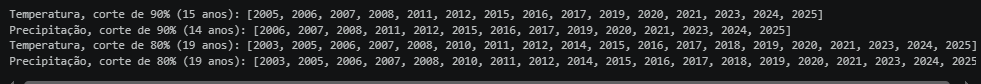
\includegraphics[width=\textwidth]{figs/anosvalidos.png}
    \caption{Anos considerados válidos sob cortes de 80\% e 90\% de dias válidos.}
    \label{fig:anos}
\end{figure}

\FloatBarrier



\subsection{Estatistica e Análise}

\subsubsection{Análise básica}

Para os dados obtidos após o processamento, foram aplicadas as funções básicas de estatistica: tamanho da amostra, média, desvio padrão, minímo, quartis e máximo. Resultados obtidos visíveis na imagem \ref{fig:estatistica}.

A análise dos resultados obtidos por essas funções aponta grande variação de temperatura e precipitação entre os anos. Nota-se que várias das medidas de \textit{std}, desvio padrão, representa uma fração uma fração significativa de \textit{mean}, média, assim como alta diferença relativa entre \textit{25\%} e \textit{75\%}, os quartis ímpares.

Apenas essas funções, não são, porém, suficientes para apontar tendência temporais de crescimento ou decrescimento dessas medidas.


\begin{figure}[htbp]
    \centering
    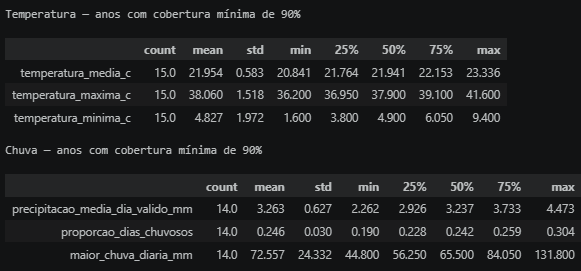
\includegraphics[width=0.85\textwidth]{figs/estatistica.png}
    \caption{Dados agrupados por anos válidos, aplicados funções básicas de estátistica.}
    \label{fig:estatistica}
\end{figure}

\FloatBarrier


\subsubsection{Análise Temporal}
\label{sec:EDAt}

Para melhor realizar a visualização e análise da evolução meteorológica da região, foram realizados \textit{plots} das medidas meteorológicas em função de tempo, visiveis nas imagens \ref{plt:temperatura}, \ref{plt:precipitacao}, \ref{plt:ciclo} e \ref{plt:boxTemp}. Os plots anuais \ref{plt:temperatura}, \ref{plt:precipitacao} e \ref{plt:boxTemp} apresentam, no escopo de estudo A705 e 2002-2025, uma tendência forte, mas inconsistente, de aumento anual da temperatura média, e redução anual de dias \textit{chuvosos}(considerados \textit{chuvosos} os dias os dias com precipitação superior a 1mm).

\begin{figure}[htbp]
    \centering
    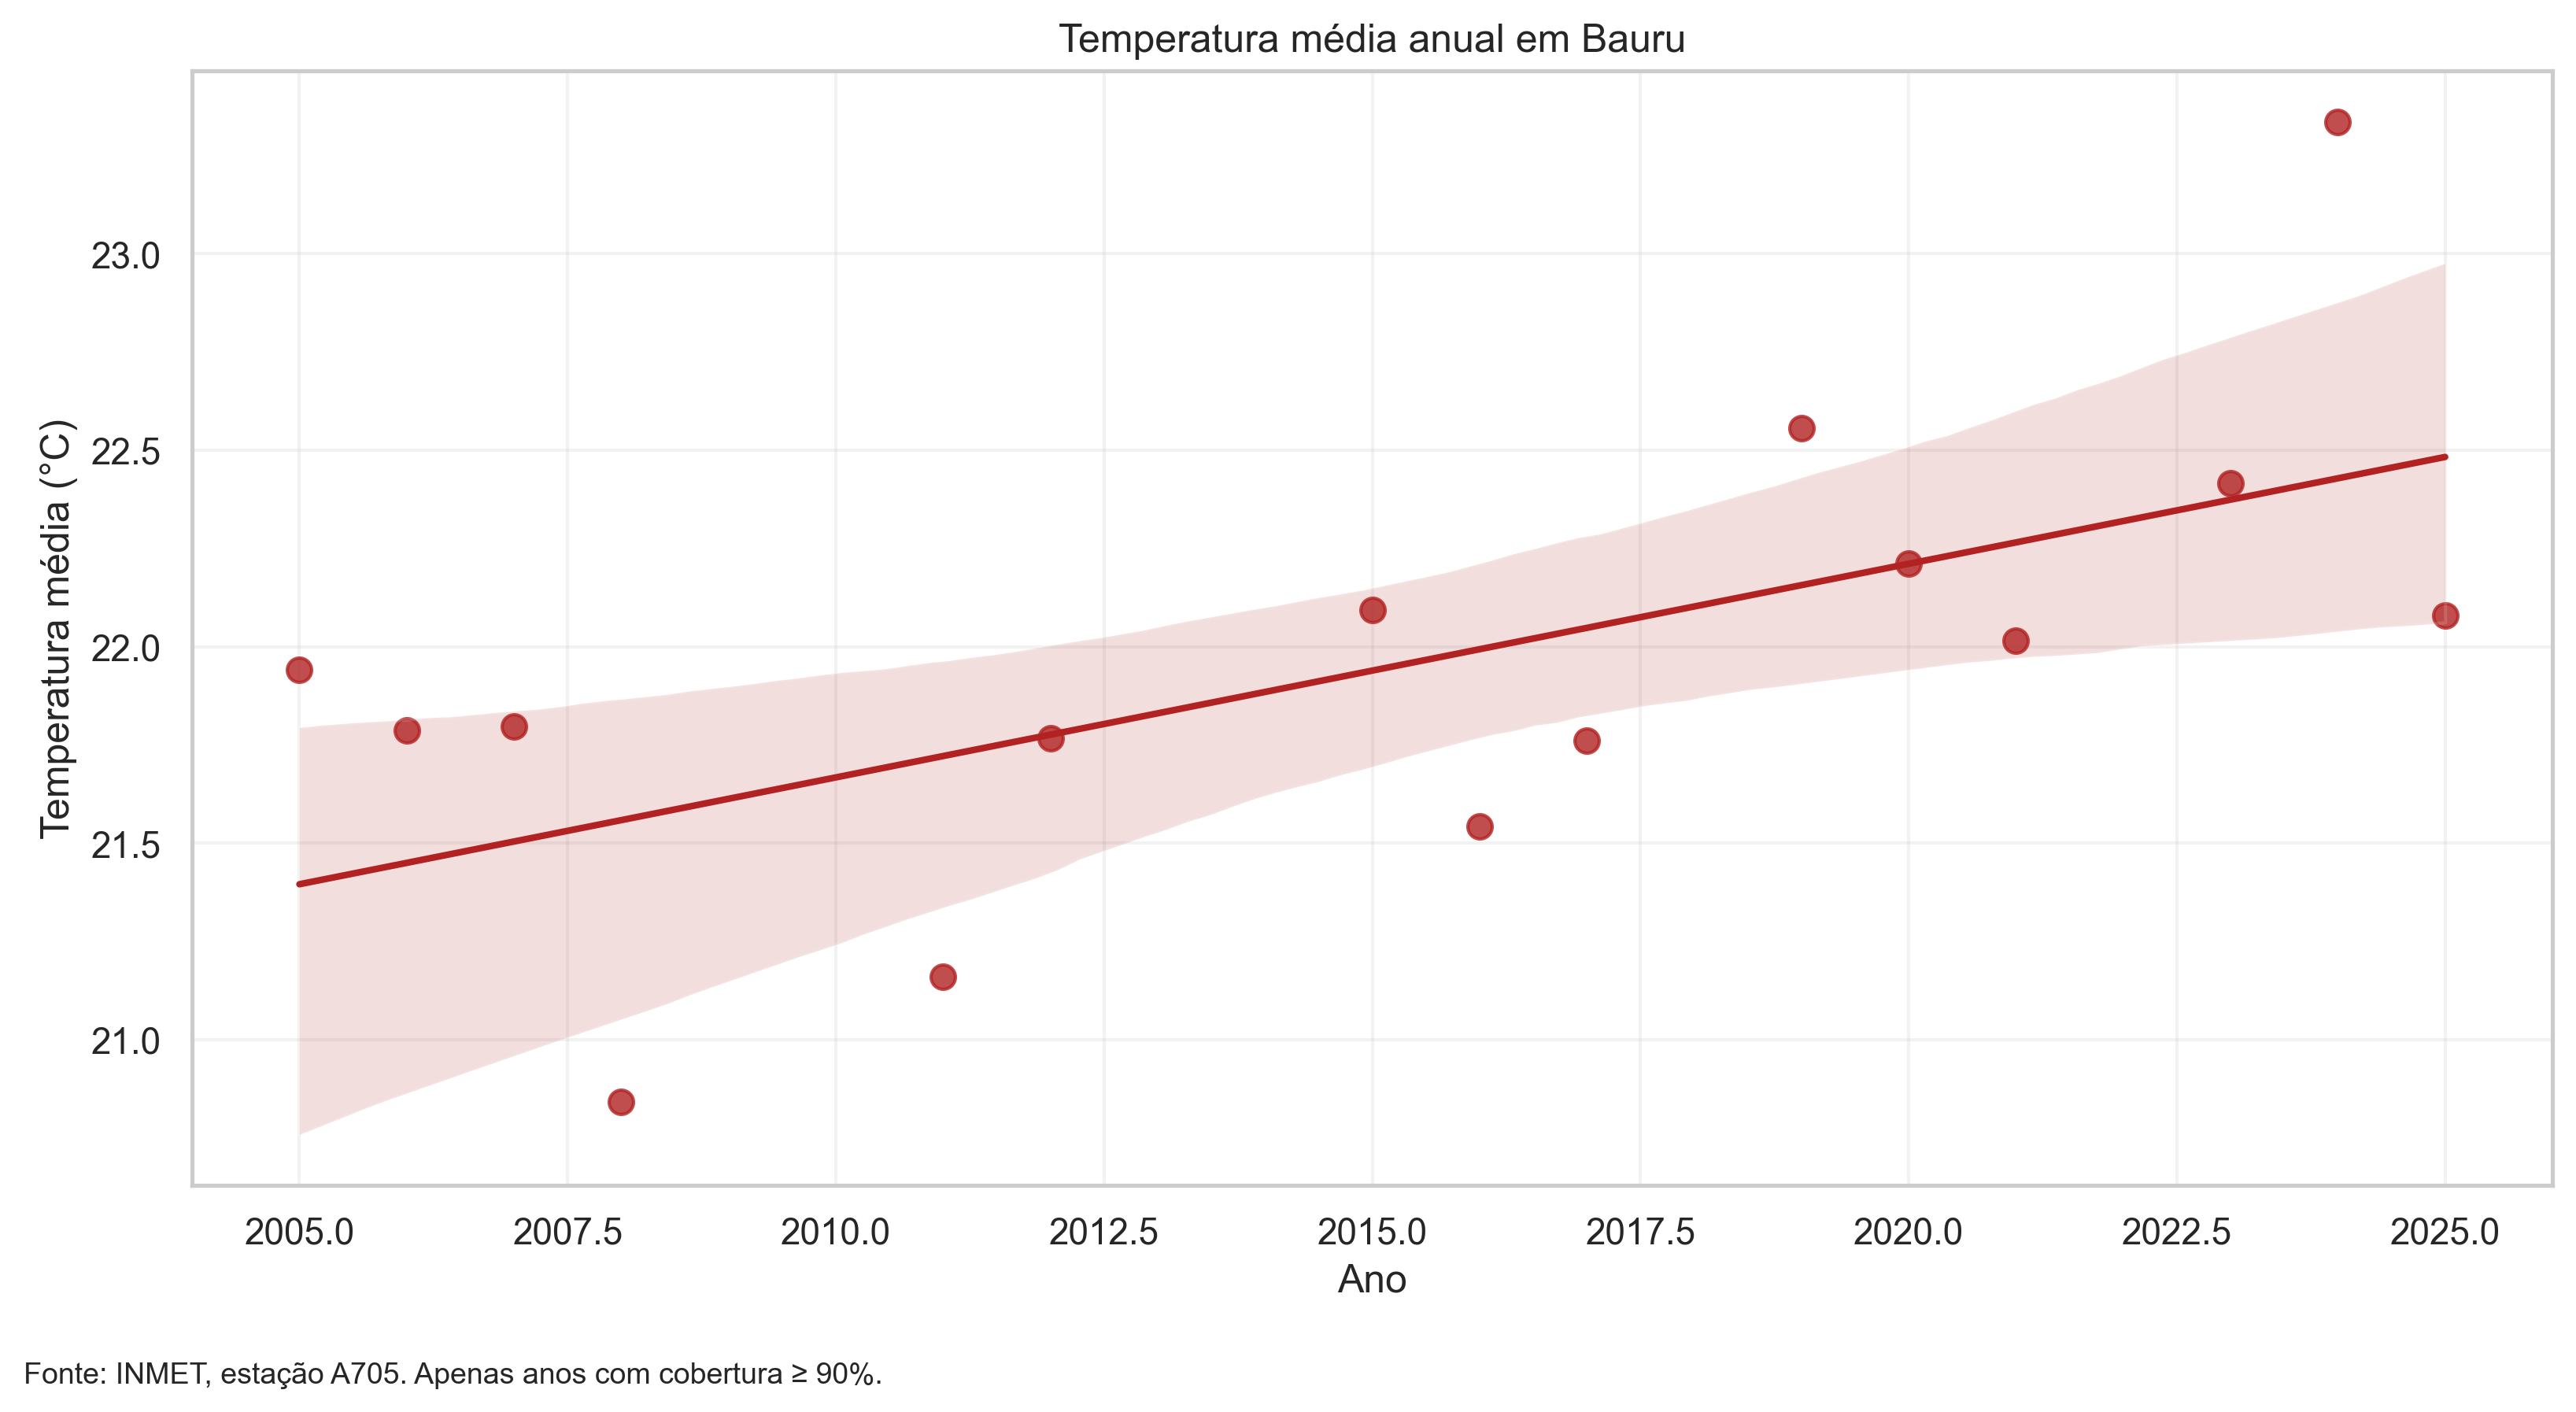
\includegraphics[width=0.8\textwidth]{figs/plot1.png}
    \caption{Evolução anual da temperatura média.}
    \label{plt:temperatura}
\end{figure}

\begin{figure}[htbp]
    \centering
    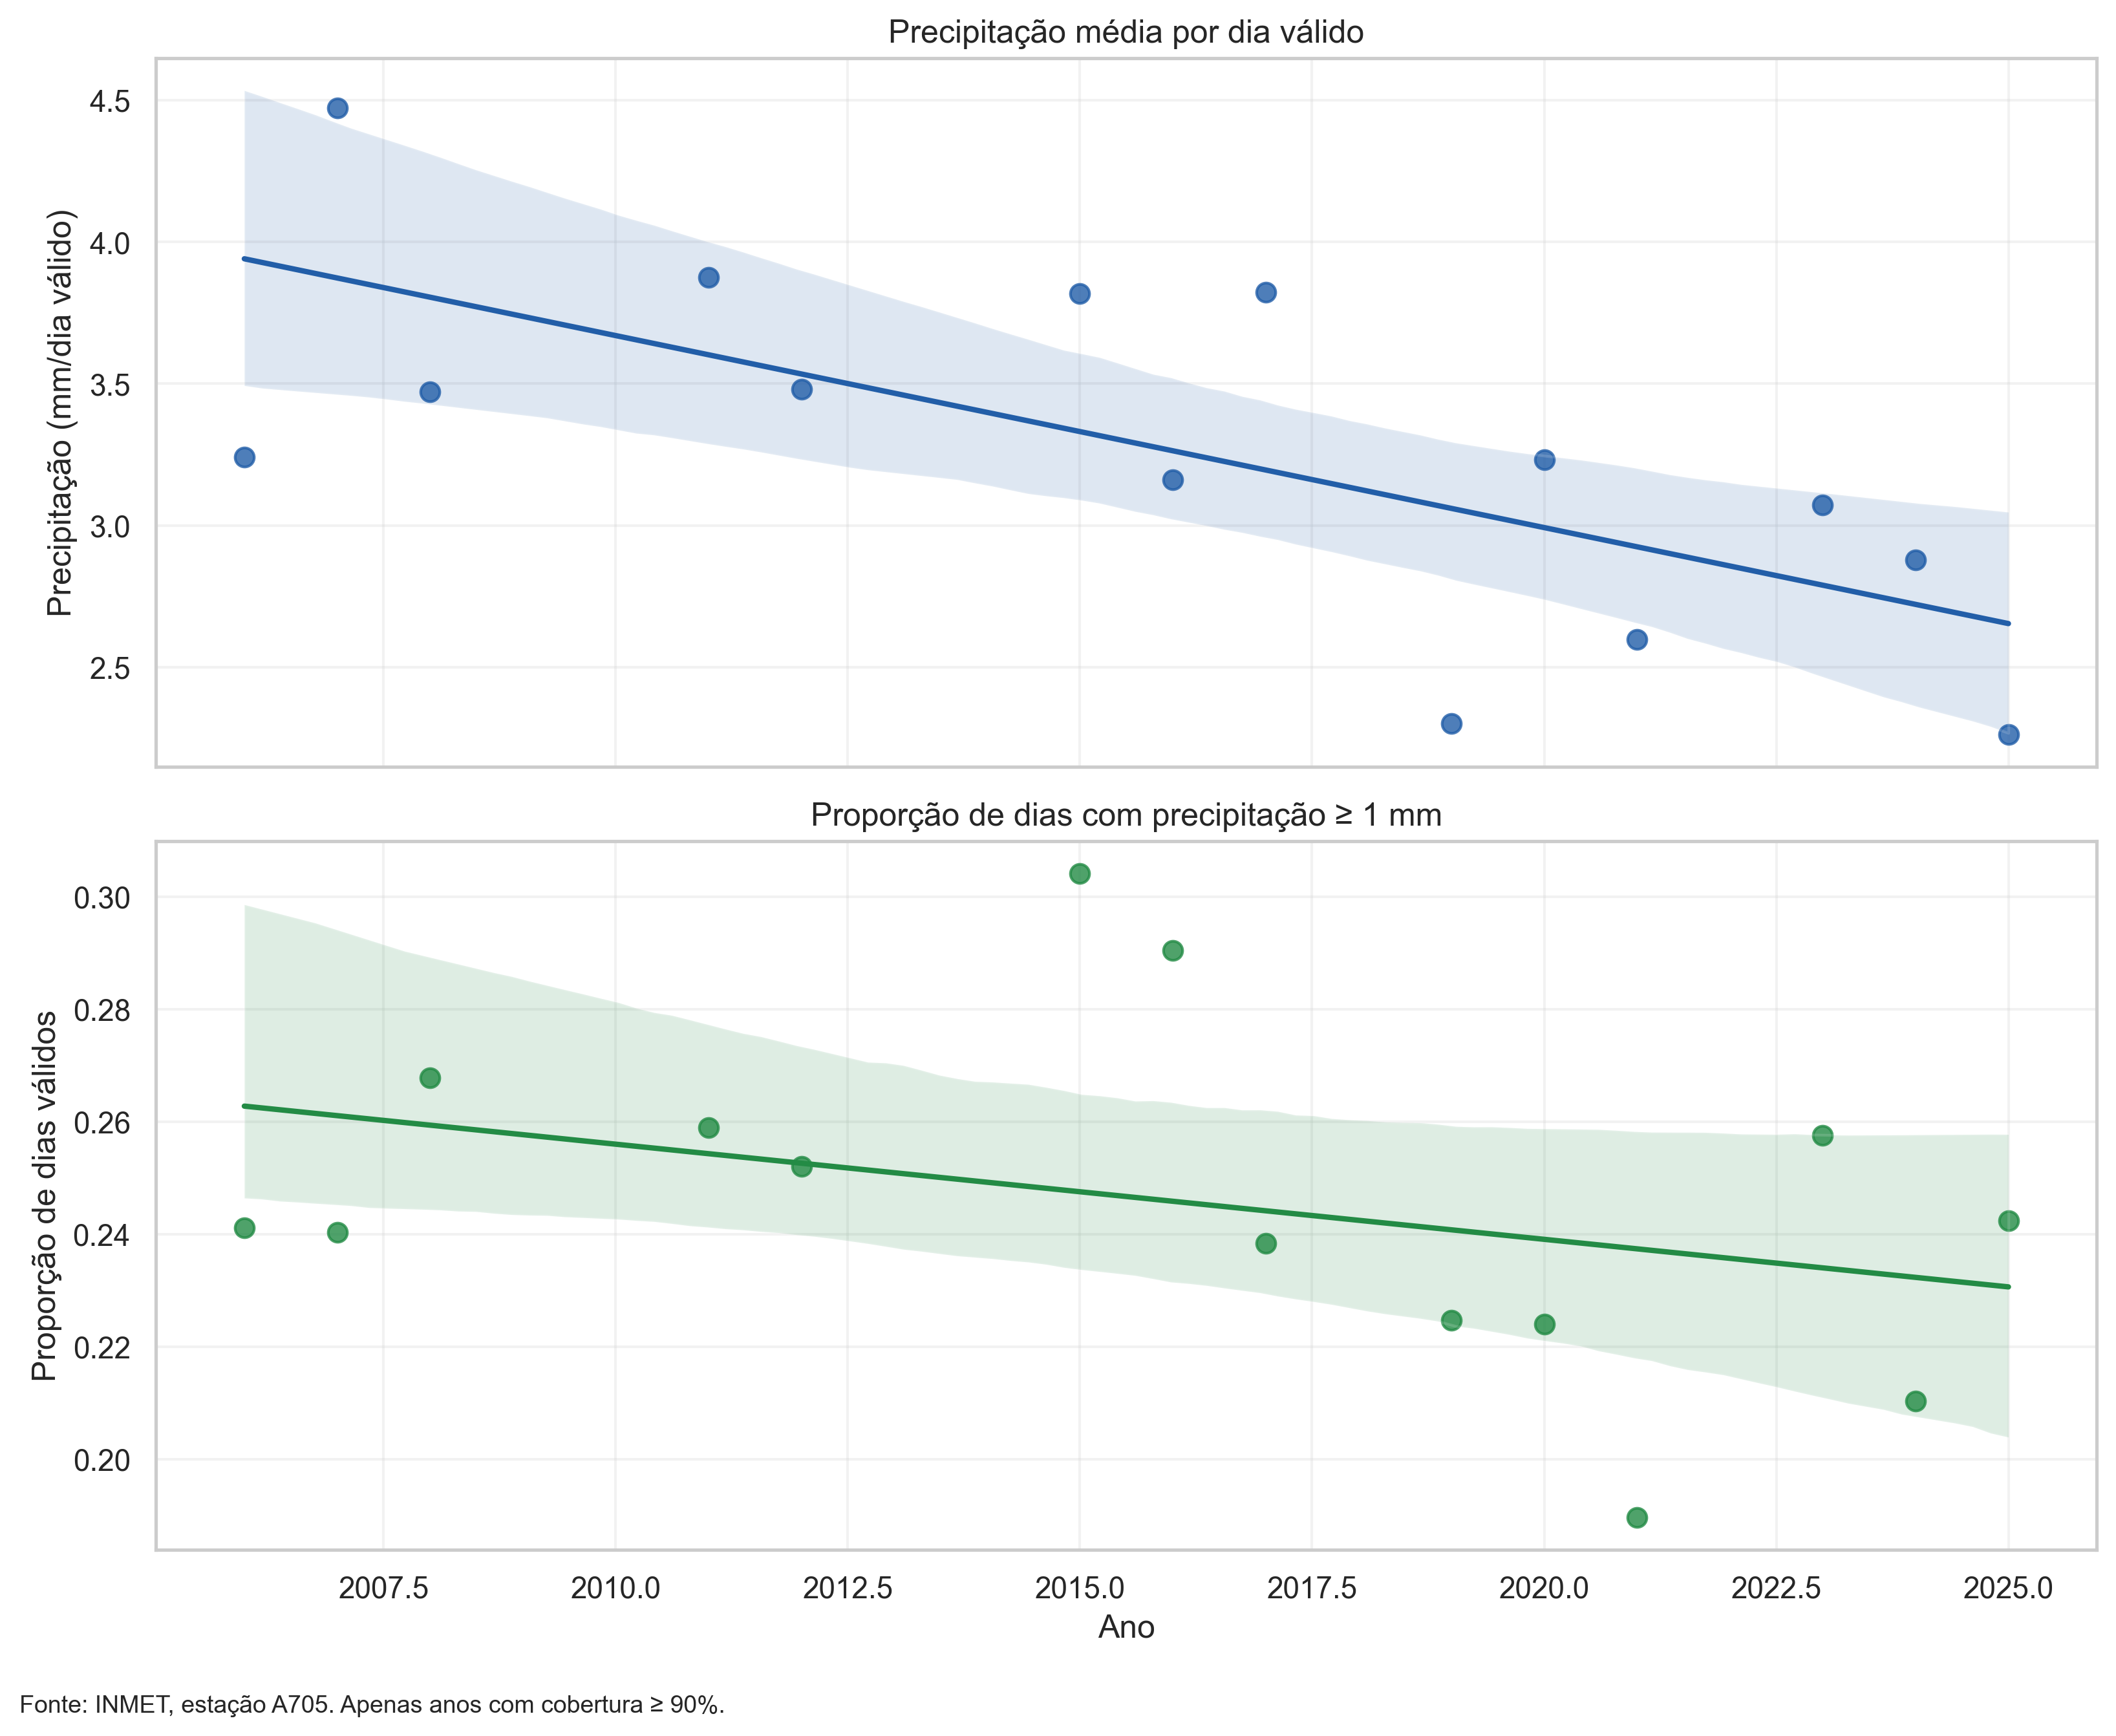
\includegraphics[width=0.8\textwidth]{figs/plot2.png}
    \caption{Evolução anual da precipitação média diária e proporção dos dias com quantidades chuva.}
    \label{plt:precipitacao}
\end{figure}

\begin{figure}[htbp]
    \centering
    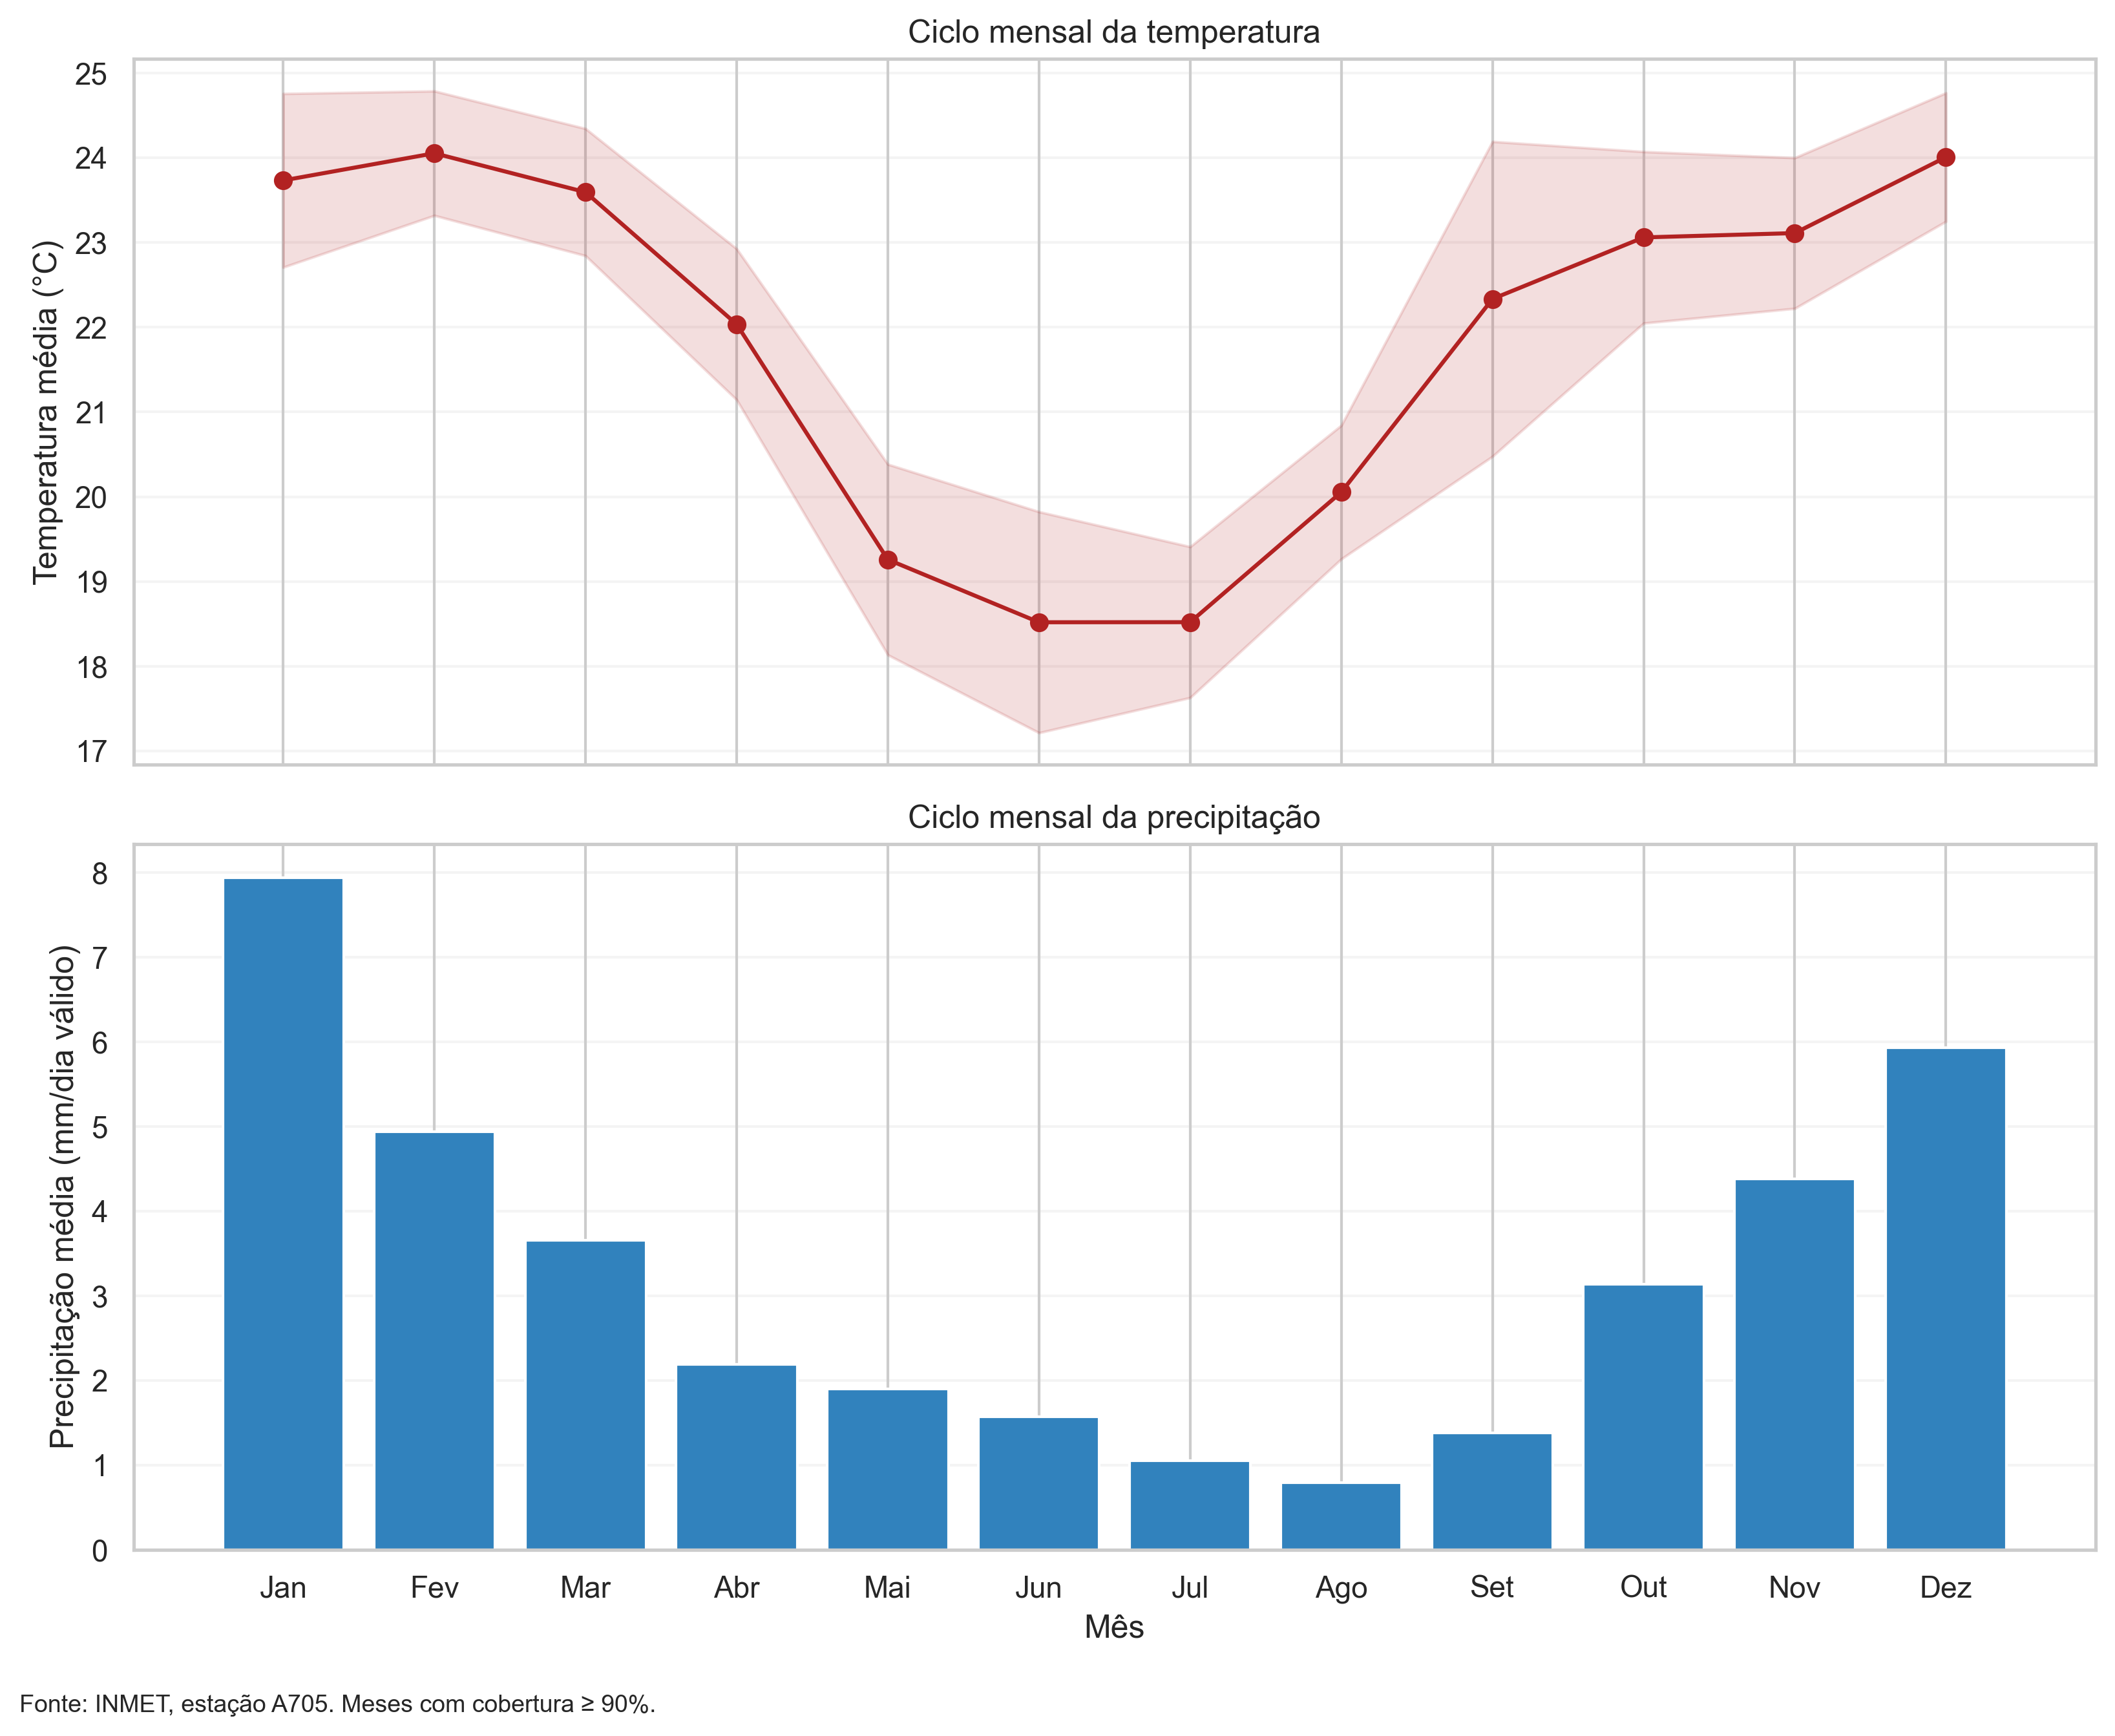
\includegraphics[width=0.8\textwidth]{figs/plot3.png}
    \caption{Variação de temperatura e precipitação em função dos meses do ano.}
    \label{plt:ciclo}
\end{figure}

\begin{figure}[htbp]
    \centering
    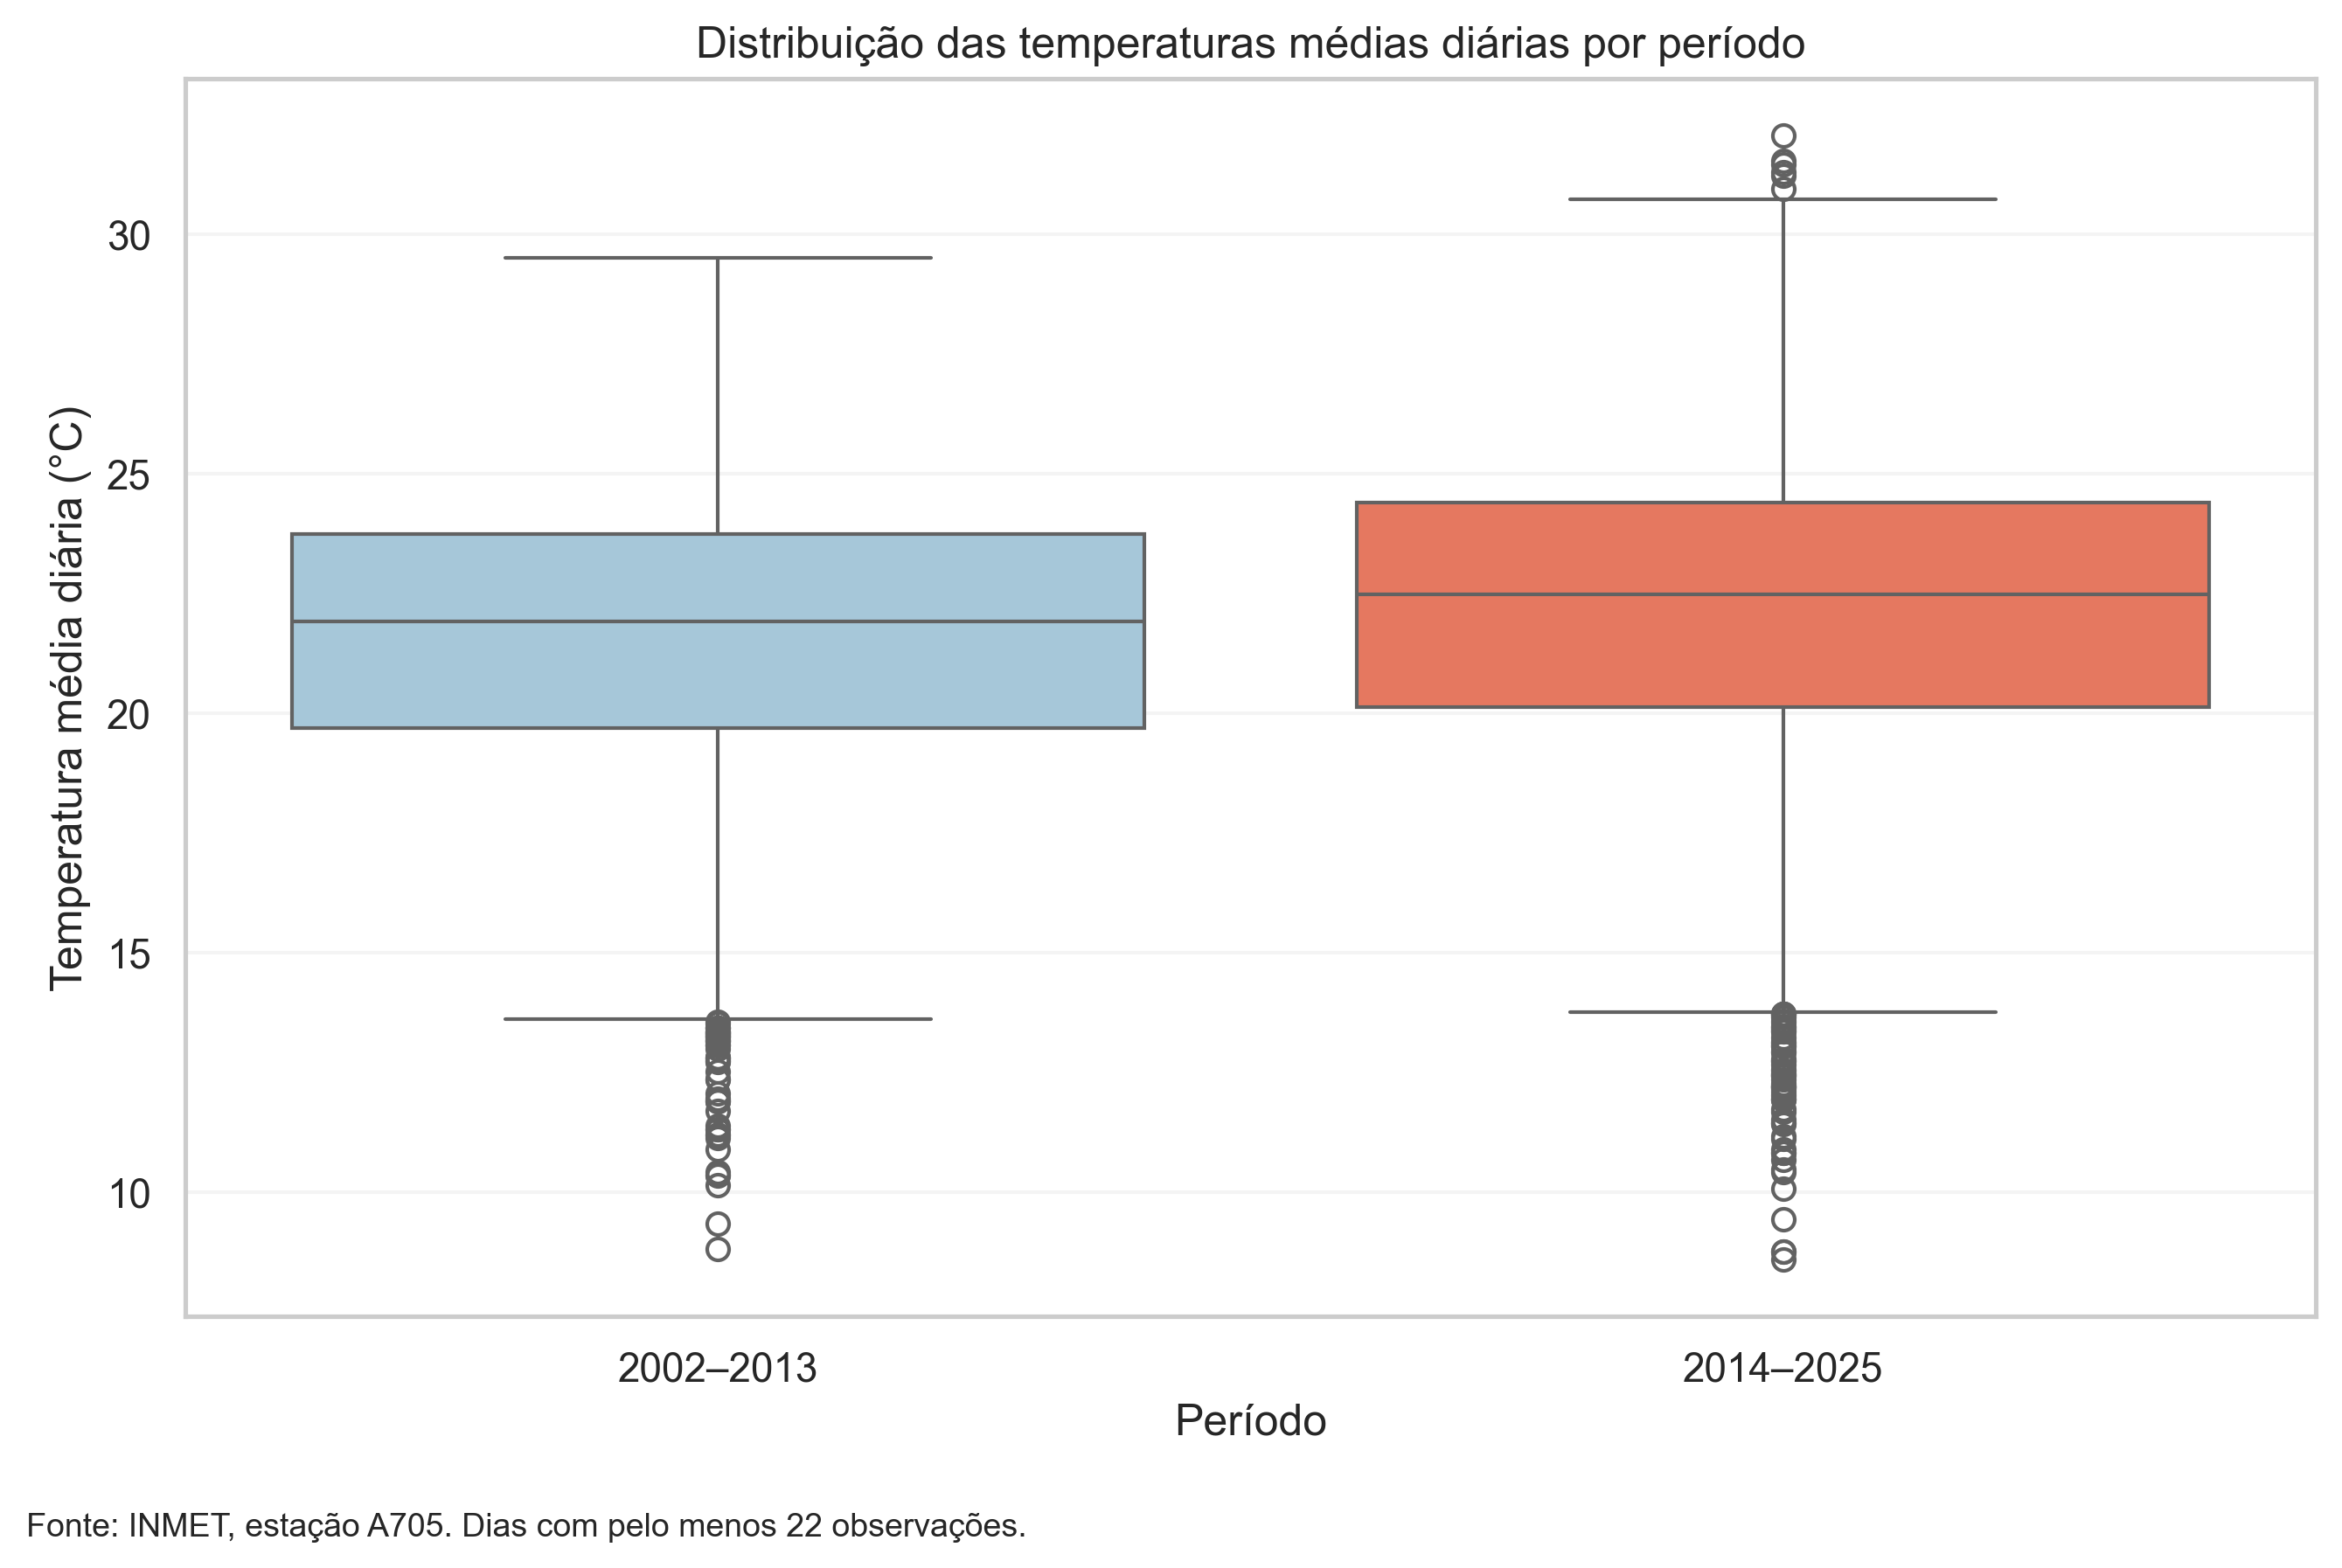
\includegraphics[width=0.8\textwidth]{figs/plot4.png}
    \caption{Box plots das temperaturas médias das metades do periodo.}
    \label{plt:boxTemp}
\end{figure}

\FloatBarrier


\subsubsection{Teste de Hipótese}
\label{sec:hip}

Para verificar formal e matemáticamente a tendência observada via plots no item \ref{sec:EDAt}, foi utilizado regressão OLS(Ordinary Least Squares) em cada indicador, para realizar teste de hipótese bilateral contra a hipótese nula de que as condições climáticas não se alteraram. Utilizou-se nível se significância de 5\% e taxa de cobertura de validação do ano de 90\% para o teste principal, e 80\% para verificação da importância da taxa de corte. Resultados visiveis na imagem \ref{fig:hipotese}.

Para a cobertura de 90\% no indicador de temperatura média anual, a regressão estimou um crescimento anual de 0.0544ºC, ou 0.54ºC por década. Essa inclinação é estatisticamente significativa ao nível de 5\%, com o valor p = 0.0113 e intervalo de confiança entre 0.14ºC e 0.94ºC por década, e logo, não incluindo 0. Esses dados apontam que o aumento de temperatura, no escopo de estudo, é muito improvável de ter acontecido aleatóriamente, aceitando a hipótese alternativa de tendência de crescimento da temperatura média. 

Por outro lado, o indicador de precipitação média diária para mesma cobertura apresenta inclinação anual estimada de redução de 0.0678mm diários. Dado o valor p de 0.0062, também se identifica inclinação estatisticamente significante, com intervalo de confiança entre -0.2315mm e -1.1236mm, não incluindo 0, formando outra aceitação da hipótese alternativa.

Apesar das outras duas análises dos indicadores, a proporção de dias chuvosos a 90\% de cobertura não aceita hipótese nula. Esse critério tem como estimativa inclinação anual negativa de 0.0017 dias, possuindo valor p alto de 0.2047 e intervalo de confiança abrangindo 0.

Ao realizar os mesmos testes com critério de anos válidos em 80\%, com o objetivo de testar a importância do valor de corte, percebeu-se que, apesar de diferenças nos valores obtidos, o resultado qualitativo se manteve o mesmo: alterar o critério não alterou sinais, não mudando as conclusões de aceitação de hipóteses nulas e alternativas. Essa característica não disprova a importância da escolha do critério, mas apenas mostra que entre ambos valores testados, não há diferenças qualitativas significantes.

Como última análise da pesquisa, realizou-se o estudo dos resíduos, Q-Q plots(Quantile-Quantile Plot) e Distância de Cook, vistos na figura \ref{fig:QQ}, para avaliar a consistência dos dados e como a pequena amostra de 14 ou 15 observações anuais pode afetar os testes de hipótese. 

Os valores registrados indicam Durbin–Watson aceitável para a maioria dos indicadores, porém atingiu 3.039 para precipitação média diária em 90\% de cobertura, apontando autocorrelação negativa forte. A distância de Cook identificou 2024 como ano influente para os modelos de temperatura, enquanto 2006 e 2007 aparecem como anos influentes no modelo de precipitação média diária. Esses diagnósticos não anulam os resultados, mas recomendam cautela ao extrapolar a inclinação para além da série observada.

\begin{figure}[htbp]
    \centering
    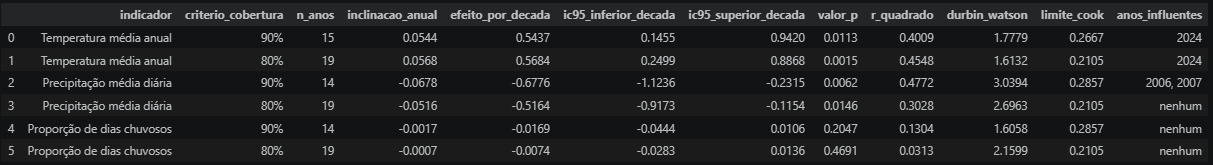
\includegraphics[width=\textwidth]{figs/testeHipotese.png}
    \caption{Tabelamento de alguns dos resultados do teste de hipótese da regressão dos indicadores.}
    \label{fig:hipotese}
\end{figure}

\begin{figure}[htbp]
    \centering
    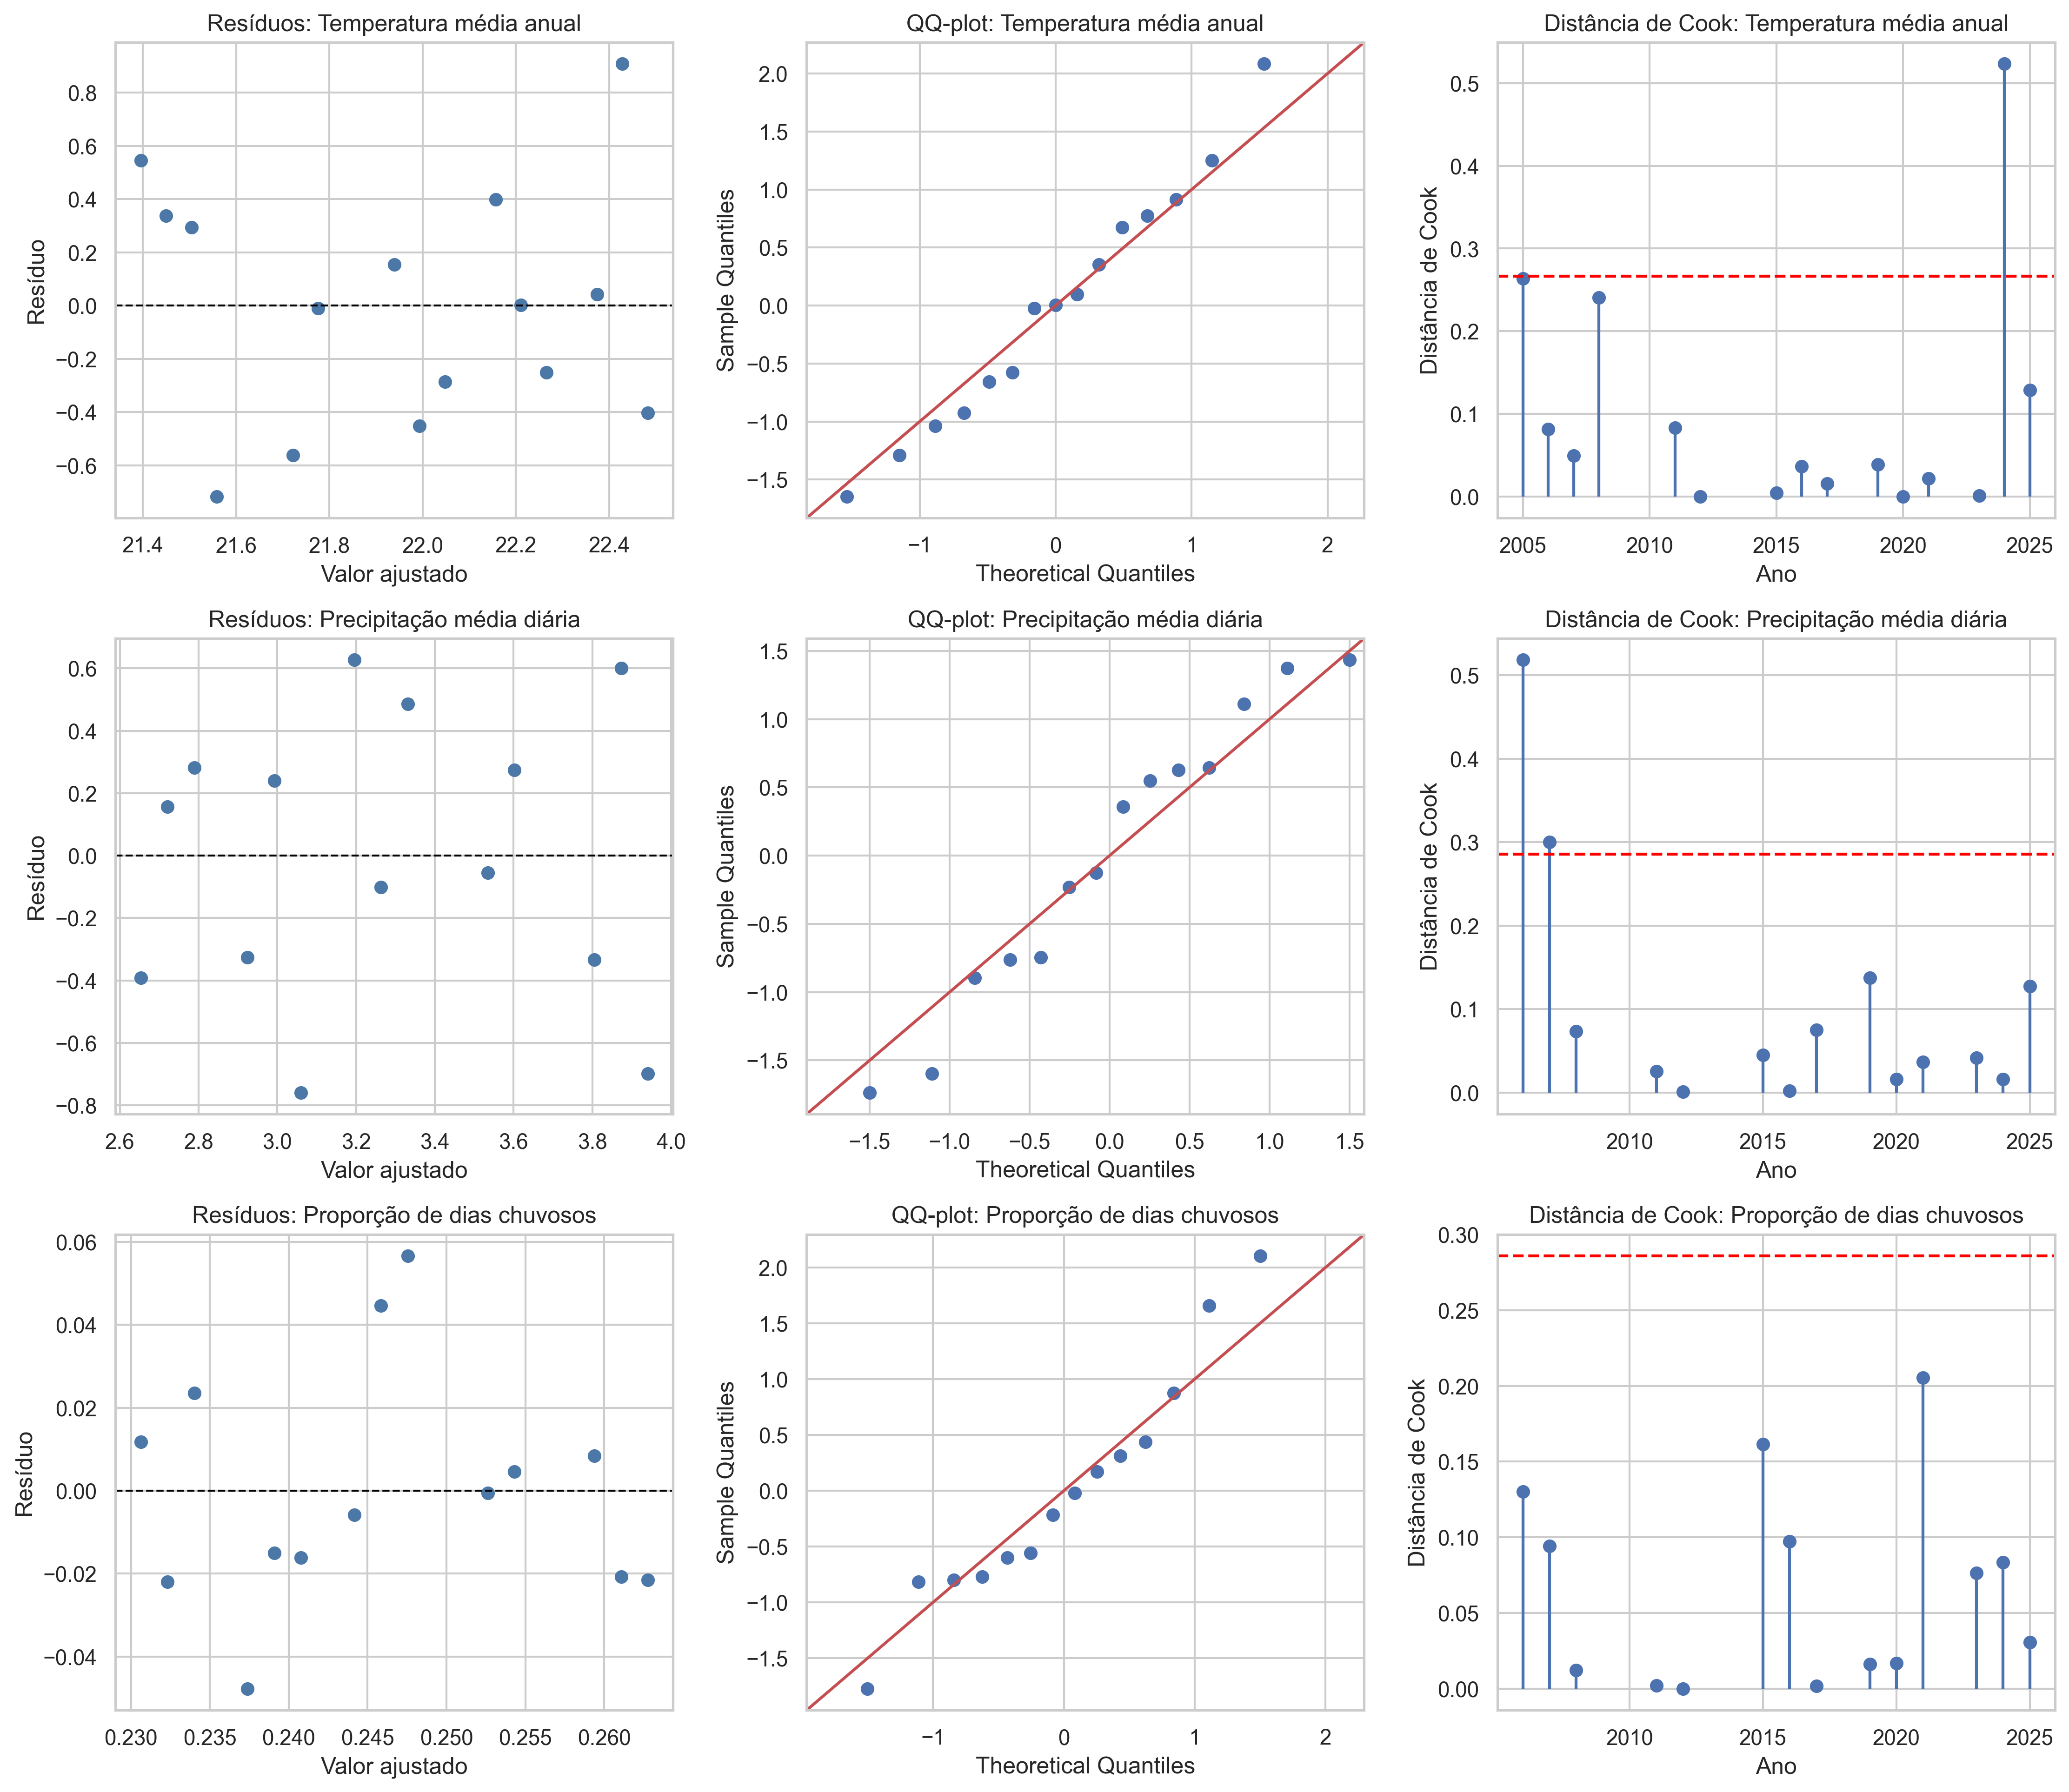
\includegraphics[width=\textwidth]{figs/plot5.png}
    \caption{Diagnósticos dos modelos principais: resíduos versus ajustados, QQ-plots e distância de Cook.}
    \label{fig:QQ}
\end{figure}



\clearpage

\section{Conclusão}

\subsection{Recomendações}

A evidência estatística de aumento da temperatura média anual e a redução de precipitação diária média é consistente entre a análise visual, o modelo OLS e a análise de sensibilidade. Porém, o aumento de temperatura e redução das chuvas nas magnitudes calculadas não são garantidas, e devem ser interpretadas como as tendências especificamente do escopo do estudo: A cidade de Bauru durante os anos de 2002 a 2025.

Mesmo com a falta de garantia dos resultados esperados, é possível apontar algumas recomendações para o planejamento urbano a médio e longo prazo, como medidas de arborização e sombreamento de áreas públicas, como em parques, pistas de caminhada e áreas de eventos, preparação de serviços e emergência para casos de insolação e desidratação, como vias de acesso exclusivo para ambulâncias e outros serviços de emergência durante meses de risco, monitoramento e fortalecimento dos reservatórios, estações de tratamento hídrico e similares, entre outros.


\subsection{Limitações}

A consideração das recomendações desse estudo deve ser feita com cautela, pois foi feita, por necessidade, utilizando dados de um período climaticamente curto de 24 anos, e apenas uma estação meteorológica automática, que esteve sujeita a falhas ou manutenções vezes o suficiente para invalidar vários dos poucos anos disponíveis para análise, e logo, afeta negativamente a confiança das conclusões.

Dado as análises da seção \ref{sec:hip}, a baixa quantidade de amostras cria uma regressão instável e altamente sucetível à \textit{outliers} em anos específicos.

Outros problemas encontrados derivam-se do fato de que as condições climáticas variam muito mais ao longo de um ano do que entre anos, como visto na imagem \ref{fig:ciclo}. Essa variabilidade sazonal não foi modelada por OLS.

Futuros estudos na área beneficiariam de um número maior de estações distribuídas pela região, assim como de maior confiabilidade do funcionamento adequado dessas, maior duração, em anos, das observações totais e modelos que englobam estações do ano.





\begin{appendices}

\section{Repositório}\label{secA1}

Link do repositório GitHub onde o código utilizado é versionado e disponibilizado:

https://github.com/GabrielNaka/DS-Projeto-Final-EDA.git

%%=============================================%%
%% For submissions to Nature Portfolio Journals %%
%% please use the heading ``Extended Data''.   %%
%%=============================================%%

%%=============================================================%%
%% Sample for another appendix section			       %%
%%=============================================================%%

%% \section{Example of another appendix section}\label{secA2}%
%% Appendices may be used for helpful, supporting or essential material that would otherwise 
%% clutter, break up or be distracting to the text. Appendices can consist of sections, figures, 
%% tables and equations etc.

\end{appendices}

%%===========================================================================================%%
%% If you are submitting to one of the Nature Portfolio journals, using the eJP submission   %%
%% system, please include the references within the manuscript file itself. You may do this  %%
%% by copying the reference list from your .bbl file, paste it into the main manuscript .tex %%
%% file, and delete the associated \verb+\bibliography+ commands.                            %%
%%===========================================================================================%%

\bibliography{sn-bibliography}% common bib file
%% if required, the content of .bbl file can be included here once bbl is generated
%%\input sn-article.bbl

\end{document}
